\documentclass[12pt]{article}

\usepackage{fancyhdr}
\usepackage{graphicx}
\usepackage{geometry}
\usepackage{lastpage}
\usepackage{titling}
\usepackage{sectsty}
\usepackage{setspace}
\usepackage{changepage}
\usepackage[shortlabels]{enumitem}
\usepackage{subcaption}
\usepackage{helvet}

\usepackage{siunitx}
\usepackage{nicefrac}
\usepackage{amsmath}
\usepackage{gensymb}
\usepackage{amssymb}
\usepackage{float}

\usepackage{listings}
\usepackage{color}
\definecolor{dkgreen}{rgb}{0,0.6,0}
\definecolor{gray}{rgb}{0.5,0.5,0.5}
\definecolor{mauve}{rgb}{0.58,0,0.82}
\lstset{
  frame=tb,
  language=MATLAB,
  aboveskip=3mm,
  belowskip=3mm,
  showstringspaces=false,
  columns=flexible,
  basicstyle={\small\ttfamily},
  numbers=none,
  numberstyle=\tiny\color{gray},
  keywordstyle=\color{blue},
  commentstyle=\color{dkgreen},
  stringstyle=\color{mauve},
  breaklines=true,
  breakatwhitespace=true,
  tabsize=3
}

\geometry
{
  letterpaper, 
  total={175.9mm,229.4mm}, 
  top=25mm, 
  left=25mm, 
  headheight=15pt,
  voffset=12pt,
  footskip=15pt
}
\author{Daniel Sturdivant}
\title{Homework 1}
\date{January 2023}
\graphicspath{ {./media/} }

\pagestyle{fancy}
\fancyhead[R]{January 30, 2023}
\fancyhead[L]{Sturdivant, Daniel}
\fancyhead[C]{MECH 6970 Intro to GPS}
\fancyfoot[C]{Page \thepage\ of \pageref{LastPage}}

\makeatletter
\def\@maketitle
{
  \null
  \begin{center}
    {\huge \@title \\}
  \end{center}
  \vskip 5mm
}
\makeatother

\sectionfont{\fontsize{16}{16}}
\subsectionfont{\fontsize{13}{13}\normalfont}
\renewcommand{\thesubsection}{\arabic{section}-\arabic{subsection}}
\renewcommand{\familydefault}{\sfdefault}
\newcommand{\solution}{\textbf{\\Solution: \\}}


%% ====================================================================== %%
\begin{document}

\maketitle
\thispagestyle{fancy}
\setstretch{1.25}
\setlength{\parskip}{0em}
\setlength{\abovedisplayskip}{-8pt}
\setlength{\belowdisplayskip}{12pt}
\setlength{\parindent}{0pt}

% \noindent\begin{tabular}{@{}ll}
%     Student: & \theauthor\\
%     Professor: &  Dr. Bevly\\
% \end{tabular}

%%
\section{Part 1}
  % 1-1
  \subsection
  {
    Given that 1 minute of latitude is approximately equal 
    to 1 nautical mile (1852 meters), how many significant digits after the 
    decimal must be included for a latitude represented in degrees to 
    describe a fix that is accurate to 1 cm? How many significant digits are 
    required after the decimal in the arc-seconds field if the latitude is 
    represented in degrees, arc-minutes, and arc-seconds to describe a fix 
    that is accurate to 1 cm? Note: 1 degree = 60 arc-minutes, 1 arc-minute = 
    60 arc-seconds (you may find arc-minutes referred to as
    'minutes' and arc-seconds referred to as 'seconds').
  } 
  \begin{adjustwidth}{10mm}{0mm}
    \solution
    \begin{equation}
      \begin{split}
        dms &= 0 \si{\degree}\quad 1 \:\si{min}\quad 0 \:\si{s} \\
        deg &= 0 \si{\degree} 
                    + \frac{1 \:\si{min}}{60 \:\si{s}}
                    + \frac{0 \:\si{s}}{3600 \:\si{s}}
                    = 0.0167 \:\si{\degree}
      \end{split}
    \end{equation}
    \\
    \begin{equation}
      \begin{split}
        \frac{dms_{1cm}}{0.01 \:\si{m}} &= 
                              \frac{1 \:\si{min}}{1852 \:\si{m}} * 
                              \frac{60 \:\si{s}}{1 \:\si{min}} \\
        dms_{1cm} &= 3(10^{-4}) \:\si{s}
      \end{split}
    \end{equation}
    \\
    \begin{equation}
      \begin{split}
        \frac{deg_{1cm}}{0.01 \:\si{m}} &= 
                              \frac{0.0167 \:\si{\degree}}{1852 \:\si{m}} \\
        dms_{1cm} &= 9(10^{-8}) \si{\degree}
      \end{split}
    \end{equation}

    As shown, the decimal precision required for sub-centimeter accuracy are 4 and 
    8 decimal places in DMS and decimal degrees respectively.
  \end{adjustwidth}

  % 1-2
  \subsection
  {
    Suppose you start from location 45° N, 120° W (lat, long) and fly at an 
    altitude of 10 km with ground speed of 885 km/hr for eight hours at a 
    constant heading of 45° from true north. Where would you end up? Assume a 
    spherical earth with radius of 6371 km. Two helpful notes: (i) Ground speed 
    in aviation means the speed of an aircraft relative to the surface of the 
    earth (to be distinguished from air speed, which means the speed of an 
    aircraft relative to its surrounding air mass). (ii) It's safe to say that 
    you'll end up pretty far north. Don't worry too much about precision -you 
    get full credit if your answer is within a kilometer of the exact answer.
  }
  \begin{adjustwidth}{10mm}{0mm}
    \solution
    Using eq. 2.111 from Groves "Principles of GNSS, Inertial, and Multisensor 
    Integrated Navigation" simplified with the assumption that the radius of the 
    Earth is constant (spherical):

    \begin{equation}
      \begin{split}
        \dot{L} &= \frac{v_{north}}{R+h} \\
        \dot{\lambda} &= \frac{v_{east}}{(R+h)\cos{L}} \\
        \dot{h} &= v_{down}
      \end{split}
    \end{equation}

    Where:

    \begin{equation}
      \begin{split}
        v &= 885 \frac{\si{km}}{\si{hr}} * \frac{1000 \:\si{m}}{1 \:\si{km}} *
                      \frac{1 \:\si{hr}}{3600 \:\si{s}} = 245.83 \frac{\si{m}}{\si{s}}\\
        v_{north} &= v * \sin{45} \\
        v_{east} &= v * \cos{45} \\
        v_{down} &= 0
      \end{split}
    \end{equation}

    Applying euler integration starting at llh = [45, -120, 10000] with a 
    dt = 1 s: \\
    \begin{equation}
      \begin{split}
        L_{k+1} &= L_{k} + dt*\dot{L}_{k} \\
        \lambda_{k+1} &= \lambda_{k} + dt*\dot{\lambda}_{k} \\
        h_{k+1} &= h_{k} + dt*\dot{h}_{k} \\
      \end{split}
    \end{equation}

    \begin{equation}
      llh_{final} = \begin{bmatrix}
        89.951535 \\[2pt] 123.494191 \\[2pt] 10000
      \end{bmatrix}
    \end{equation}

    \begin{figure}[H]
      \centering
      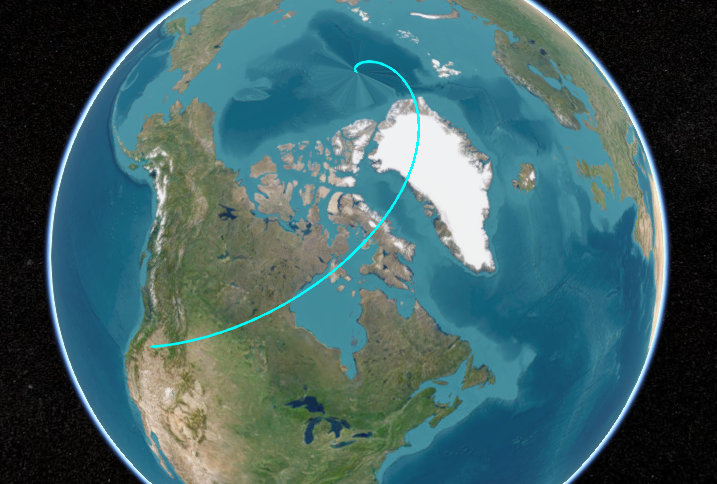
\includegraphics[width=0.7\textwidth]{path_1-3.png}
      \caption{Path of the Aircraft.}
    \end{figure}
  \end{adjustwidth}

  % 1-3
  \subsection
  {
    An aircraft is carrying a transmitter that is broadcasting a single tone at 
    100 MHz. The aircraft flies away from you on a straight line at constant 
    altitude with ground speed of 360 km/hr. You measure the following Doppler 
    shifts from 100 MHz spaced 0.1 s apart: -33.1679 Hz, -33.1711 Hz, and 
    -33.1743 Hz. Determine the range rates in m/s that correspond to these 
    Doppler measurements. In the figure below, the aircraft altitude is $Y_0$: and 
    its horizontal distance from observer at the three instants of Doppler 
    measurements is shown as $X_0$, $X_1$, and $X_2$, respectively. Set up two linear 
    equations that relate $X_1$ and $X_2$, to $X_0$. Can you set up two non-linear 
    equations that relate $X_0$ and $Y_0$ to the measurements? For extra credit, 
    solve the equations iteratively.
  }
  \begin{adjustwidth}{10mm}{0mm}
    \solution
    \begin{equation}
      \begin{split}
        f_{R} &= f_{T}(1 - \frac{\dot{r}}{v_{s}}) \\
        \dot{r} &= \frac{v_{s}}{f_{T}}(f_{R} - f_{T})
      \end{split}
    \end{equation}

    Substituting in $v_s = 3(10^8)$ m/s (speed of light), $f_{T} = 100(10^6)$ Hz, 
    and $f_{R} - f_{T} =$ the measured doppler shifts:

    \begin{equation}
      \dot{r} = \begin{bmatrix}
        99.503700 \\[2pt] 99.513300 \\[2pt] 99.522900
      \end{bmatrix}
      \frac{\si{m}}{\si{s}}
    \end{equation}

    The two linear equations are the equations for a constant velocity vehicle
    with $v = 360$ km/hr $= 100$ m/s.
    
    \begin{equation}
      \begin{split}
        x_1 &= x_0 + v*dt = x_0 + (360*\frac{1000}{3600})*0.1 = x_0 + 10 \\
        x_2 &= x_0 + v*dt = x_0 + (360*\frac{1000}{3600})*0.2 = x_0 + 20
      \end{split}
    \end{equation}

    The nonlinear equations were derived as followed:

    \begin{equation}
      \begin{split}
        r_0 &= \sqrt{x_0^2 + y_0^2} \\
        r_0^2 &= x_0^2 + y_0^2 \\
        2r_0\dot{r_0} &= 2x_0\dot{x_0} + 2y_0\dot{y_0} \\
        \dot{r_0} &= \frac{x_0\dot{x_0}}{r_0} = \frac{x_0v}
                                                {\sqrt{x_0^2 + y_0^2}}
      \end{split}
    \end{equation}

    Similarly the equations for $\dot{r_1}$ and $\dot{r_2}$ as functions of 
    $x_0$ and $y_0$:

    \begin{equation}
      \begin{split}
        \dot{r_1} &= \frac{x_1\dot{x_1}}{r_1} = \frac{(x_0+10)v}
                                                {\sqrt{(x_0+10)^2 + y_0^2}} \\
        \dot{r_2} &= \frac{x_2\dot{x_2}}{r_2} = \frac{(x_0+20)v}
                                                {\sqrt{(x_0+20)^2 + y_0^2}} \\
      \end{split}
    \end{equation}

    To solve for $X_0$ and $Y_0$ iteratively, a jacobian matrix and 
    measurement vector must be made a follows:

    \begin{equation}
      \begin{split}
        \dot{r_0} &= \hat{\dot{r_0}} + \frac{\partial{\dot{r}}}{\partial{y_0}}
        (y_0 - \hat{y}) + \frac{\partial{\dot{r}}}{\partial{x_0}}(x_0 - \hat{x}) \\
        \dot{r_1} &= \hat{\dot{r_1}} + \frac{\partial{\dot{r}}}{\partial{y_1}}
        (y_1 - \hat{y}) + \frac{\partial{\dot{r}}}{\partial{x_1}}(x_1 - \hat{x}) \\
        \dot{r_2} &= \hat{\dot{r_0}} + \frac{\partial{\dot{r}}}{\partial{y_2}}
        (y_2 - \hat{y}) + \frac{\partial{\dot{r}}}{\partial{x_2}}(x_1 - \hat{x}) \\
      \end{split}
    \end{equation}

    Using both the linear and nonlinear equations, the resulting system is:

    \begin{equation}
      \begin{split}
        H &= \begin{bmatrix}
          \dfrac{100y_0^2}{(x_0^2 + y_0^2)^\frac{3}{2}} &
          \dfrac{-100x_0y_0}{{(x_0^2 + y_0^2)^\frac{3}{2}}} \\[20pt]
          \dfrac{100y_0^2}{((x_0+10)^2 + y_0^2)^\frac{3}{2}} &
          \dfrac{-100(x_0+10)y_0}{{((x_0+10)^2 + y_0^2)^\frac{3}{2}}} \\[20pt]
          \dfrac{100y_0^2}{((x_0+20)^2 + y_0^2)^\frac{3}{2}} &
          \dfrac{-100(x_0+20)y_0}{{((x_0+20)^2 + y_0^2)^\frac{3}{2}}}
        \end{bmatrix} \\ \\
        y &= \dot{r} - \hat{\dot{r}} = 
        \begin{bmatrix}
          99.503700 - \hat{\dot{r_0}} \\[2pt] 
          99.513300 - \hat{\dot{r_1}} \\[2pt]
          99.522900 - \hat{\dot{r_2}} 
        \end{bmatrix} \\ \\
        \Delta x &= \begin{bmatrix}
          x_0 - \hat{x_0} \\[2pt]
          y_0 - \hat{y_0}
        \end{bmatrix} \\
        \\
        y &= H \Delta x \\
        \Delta x &= (H^T H)^{-1} H^T y
      \end{split}
    \end{equation}

    This can be iteratively solved by consecutively adding $\Delta x$ to the 
    current estimate of $x$ until the error is considered negligible.
  \end{adjustwidth}

  % 1-4
  \subsection
  {
    A pseudolite (short for pseudo-satellite) consists of a generator of a GPS-like 
    signal and a transmitter. Pseudolites are used to augment the GPS signals. 
    Suppose an observer is constrained to be on the line joining two pseudolites 
    PL1 and PL2, which are separated by 1 km. The pseudolite clocks are perfectly 
    synchronized but the observer's clock may have an unknown bias with respect to 
    the pseudolite clocks. Estimate the observer's position and clock bias given 
    that the pseudoranges to PL1 and PL2 are (a) 550 m and 500 m, respectively, and 
    (b) 400 m and 1400 m, respectively.
  }
  \begin{adjustwidth}{10mm}{0mm}
    \solution
    Using the equation for psuedoranges:

    \begin{equation}
      \begin{split}
        \rho_1 &= \sqrt{(x_1 - x)^2} - b = \sqrt{(0-x)^2} - b = \sqrt{x^2} - b \\
        \rho_2 &= \sqrt{(x_2 - x)^2} - b = \sqrt{(1000 - x)^2} - b \\ \\
        -x + b &= 0 - \rho_1 \\
        x + b  &= 1000 - \rho_1
      \end{split}
    \end{equation}

    Solving a system of two linear equations:

    \begin{equation}
      \begin{split}
        \begin{bmatrix}
          0 - \rho_1 \\ 1000 - \rho_2 
        \end{bmatrix}
        &=
        \begin{bmatrix}
          -1 & 1 \\ 1 & 1
        \end{bmatrix}
        \begin{bmatrix}
          x \\ b
        \end{bmatrix} 
        \\
        \begin{bmatrix}
          x \\ b 
        \end{bmatrix}
        &=
        \begin{bmatrix}
          -1 & 1 \\ 1 & 1
        \end{bmatrix}^{-1}
        \begin{bmatrix}
          0 - \rho_1 \\ 1000 - \rho_2
        \end{bmatrix} 
        \\
        \begin{bmatrix}
          x \\ b 
        \end{bmatrix}
        &=
        \begin{bmatrix}
          -1 & 1 \\ 1 & 1
        \end{bmatrix}^{-1}
        \begin{bmatrix}
          0 - 550 \\ 1000 - 500
        \end{bmatrix}
        =
        \begin{bmatrix}
          525 \\ -25
        \end{bmatrix} \si{m}
        \\
        \begin{bmatrix}
          x \\ b 
        \end{bmatrix}
        &=
        \begin{bmatrix}
          -1 & 1 \\ 1 & 1
        \end{bmatrix}^{-1}
        \begin{bmatrix}
          0 - 400 \\ 1000 - 1400
        \end{bmatrix}
        =
        \begin{bmatrix}
          0 \\ -400
        \end{bmatrix} \si{m}
      \end{split}
    \end{equation}
  \end{adjustwidth}

  %%
  \vspace{16pt}
  \section{Part 2}
    \subsection*
    {
      Generate two random sequences of length 100 and randomly comprised of +1 and -1.
      \begin{enumerate}[(a)]
        \itemsep -6pt
        \item Plot the histogram on each sequence.
        \item Plot the spectral analysis on each sequence.
        \item Plot the autocorrelation of each sequence with itself.
        \item Plot the cross correlation between the two sequences.
        \item BONUS: Repeat for a sequence that is 1000 long and compare to the above.
      \end{enumerate}
    }

    \solution
    The two sequences were created using the following MATLAB commands: \\
    \begin{equation}
      \begin{split}
        seq1 &= 2*\si{ceil}(\si{rand}(100,1)-0.5)-1 \\
        seq2 &= 2*\si{ceil}(0.1*\si{randn}(100,1))-1
      \end{split}
    \end{equation}

    \vspace{12pt}
    Resulting in the following histograms:

    \begin{figure}[H]
      \centering
      \begin{minipage}{0.5\textwidth}
        \centering
        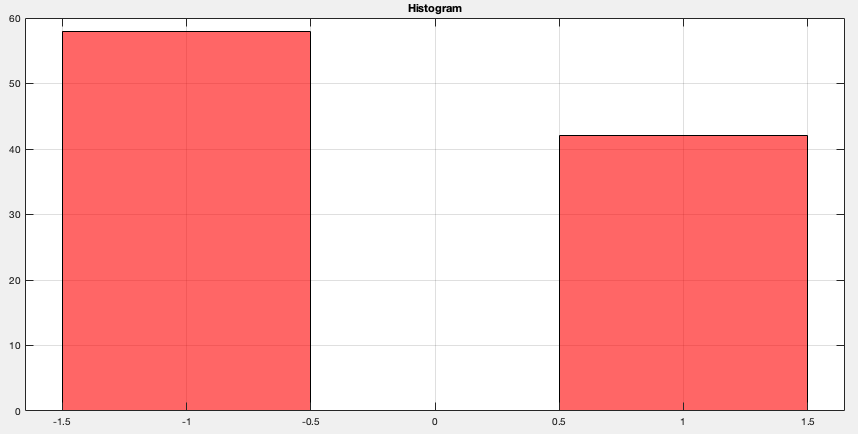
\includegraphics[width=0.95\textwidth]{seq1_hist.png}
        \captionof{figure}{Sequence 1 Histogram.}
      \end{minipage}%
      \begin{minipage}{0.5\textwidth}
        \centering
        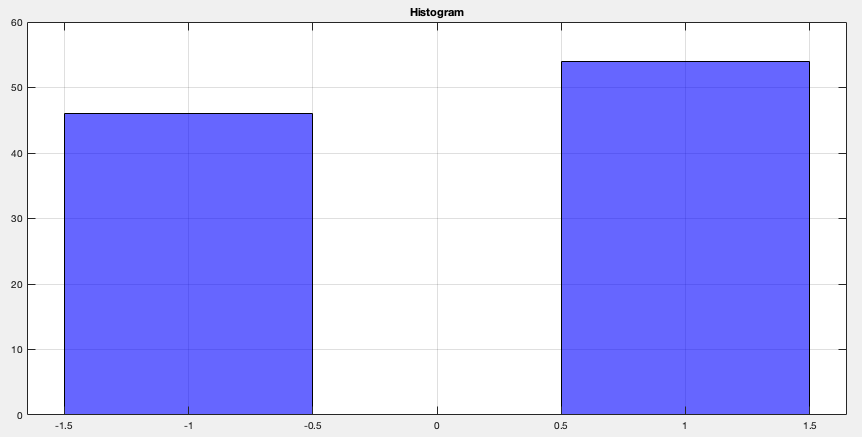
\includegraphics[width=0.95\textwidth]{seq2_hist.png}
        \captionof{figure}{Sequence 2 Histogram.}
      \end{minipage}
    \end{figure}

    \vspace{10pt}
    Using the MATLAB command $abs(fft(seq))$ to get the power spectral density 
    of each sequence and plotting the output:

    \begin{figure}[H]
      \centering
      \begin{minipage}{0.5\textwidth}
        \centering
        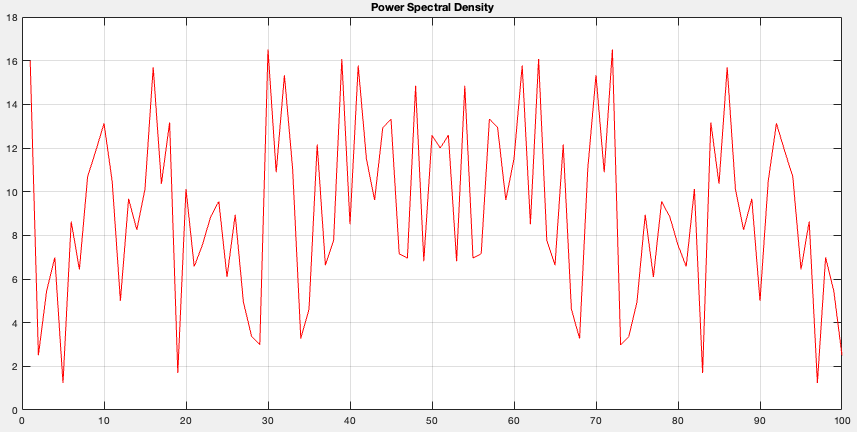
\includegraphics[width=0.95\textwidth]{seq1_psd.png}
        \captionof{figure}{Sequence 1 PSD.}
      \end{minipage}%
      \begin{minipage}{0.5\textwidth}
        \centering
        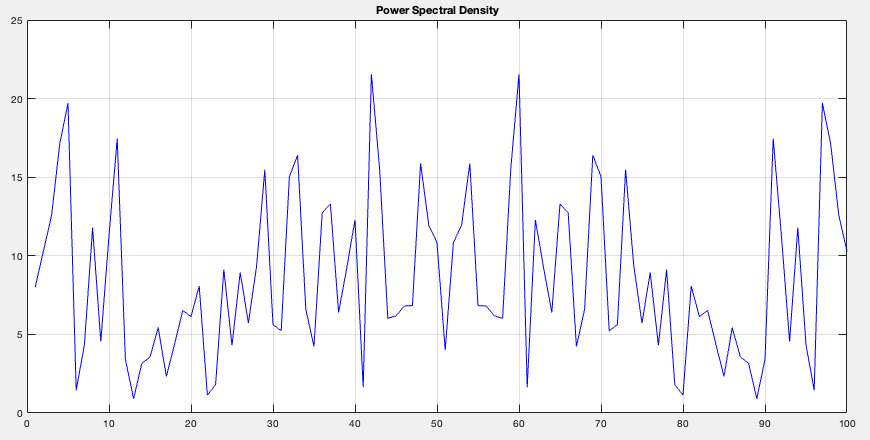
\includegraphics[width=0.95\textwidth]{seq2_psd.png}
        \captionof{figure}{Sequence 2 PSD.}
      \end{minipage}
    \end{figure}

    \vspace{10pt}
    Next a MATLAB function was made for the correlation of different sequences.

    \begin{lstlisting}
    function [R, shifts] = correlation(seq1, seq2)
      if size(seq1) ~= size(seq2)
        fprintf('ERROR: "correlation" -> sequneces not the same size!');
        return;
      end

      N = length(seq1);
      shifts = -(N-1):(N-1);
      R = zeros([length(shifts),1]);

      for k = 1:length(shifts)
        seq1_ = circshift(seq1, shifts(k));
        R(k) = 1/N * sum(seq1_.*seq2);
      end
    end
    \end{lstlisting}

    \vspace{10pt}
    This function outputs the following autocorrelations, showing that each 
    sequence is only correlated with itself when there is no shift in the 
    sequence:

    \begin{figure}[H]
      \centering
      \begin{minipage}{0.5\textwidth}
        \centering
        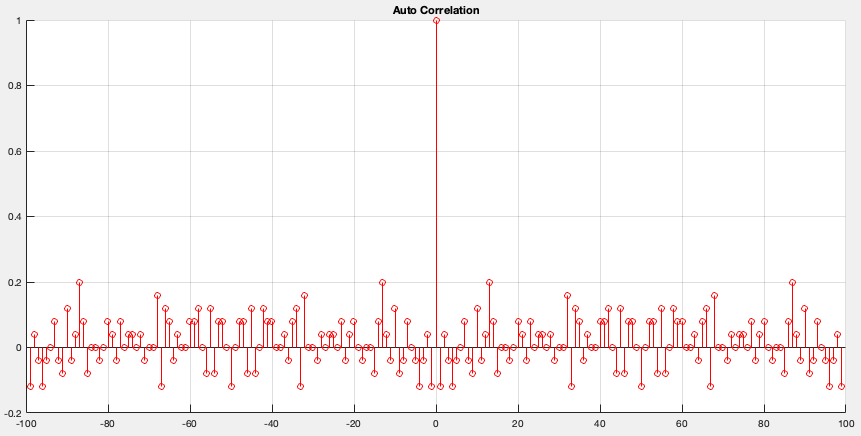
\includegraphics[width=0.95\textwidth]{seq1_xcorr.png}
        \captionof{figure}{Sequence 1 Autocorrelation.}
      \end{minipage}%
      \begin{minipage}{0.5\textwidth}
        \centering
        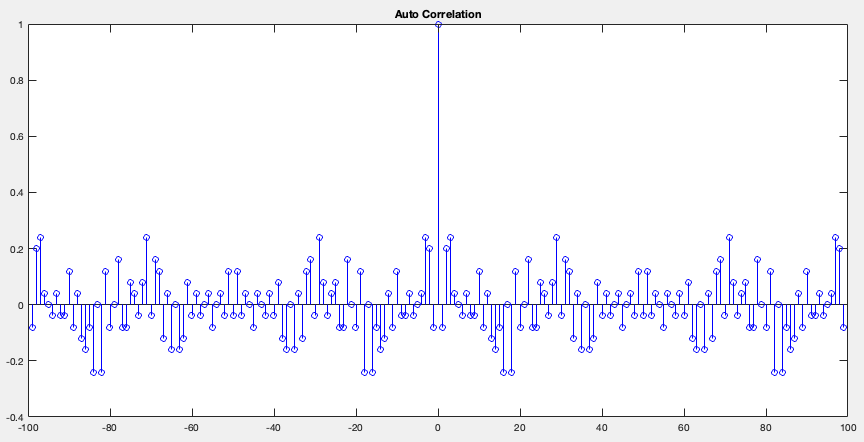
\includegraphics[width=0.95\textwidth]{seq2_xcorr.png}
        \captionof{figure}{Sequence 2 Autocorrelation.}
      \end{minipage}
    \end{figure}

    \vspace{10pt}
    Using the same function to find the crosscorrelation of the sequences, 
    there is no correlation:

    \begin{figure}[H]
      \centering
      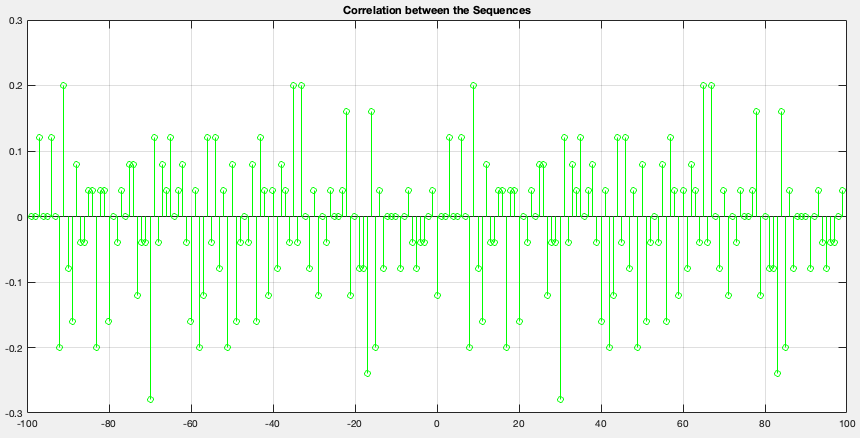
\includegraphics[width=0.5\textwidth]{xcorr.png}
      \caption{Crosscorrelation of the Sequences.}
    \end{figure}

    \vspace{10pt}
    Repeating all the steps above for a sequence of length 1000.

    \begin{figure}[H]
      \centering
      \begin{minipage}{0.5\textwidth}
        \centering
        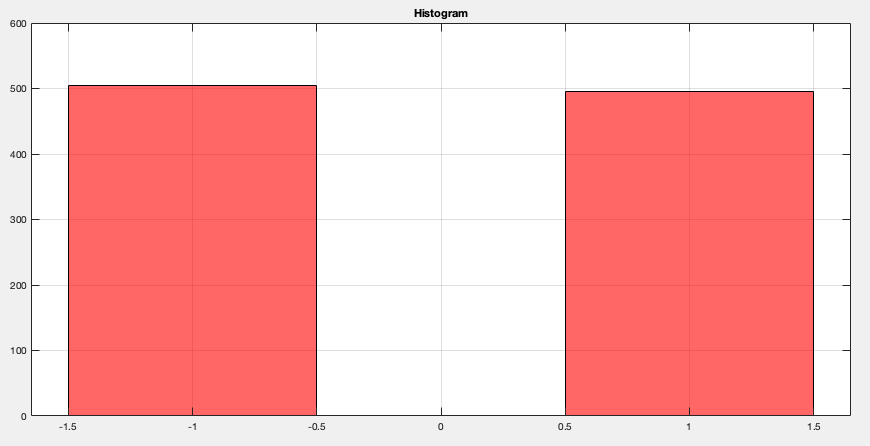
\includegraphics[width=0.95\textwidth]{seq1_1000_hist.png}
        \captionof{figure}{Sequence 1 Histogram.}
      \end{minipage}%
      \begin{minipage}{0.5\textwidth}
        \centering
        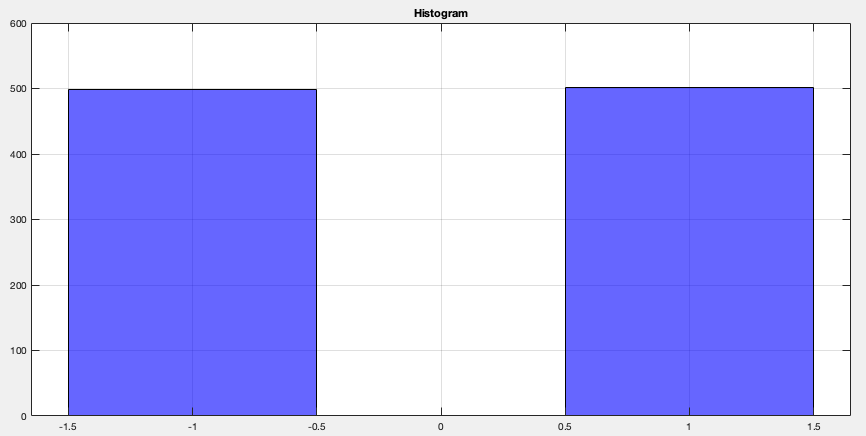
\includegraphics[width=0.95\textwidth]{seq2_1000_hist.png}
        \captionof{figure}{Sequence 2 Histogram.}
      \end{minipage}
    \end{figure}

    \begin{figure}[H]
      \centering
      \begin{minipage}{0.5\textwidth}
        \centering
        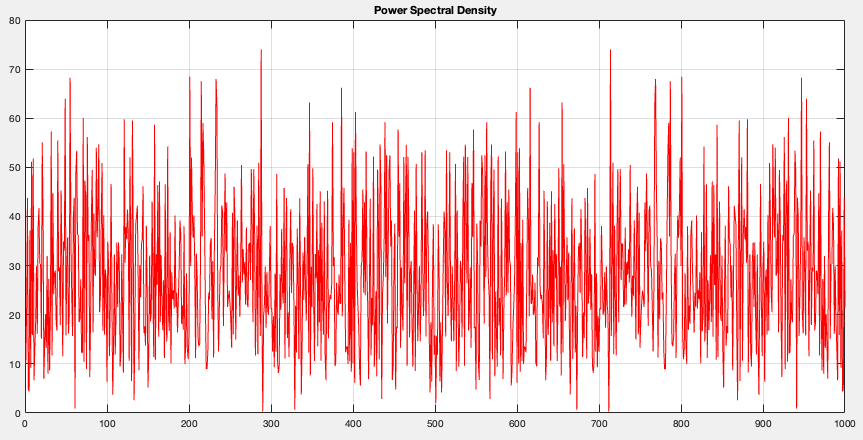
\includegraphics[width=0.95\textwidth]{seq1_1000_psd.png}
        \captionof{figure}{Sequence 1 PSD.}
      \end{minipage}%
      \begin{minipage}{0.5\textwidth}
        \centering
        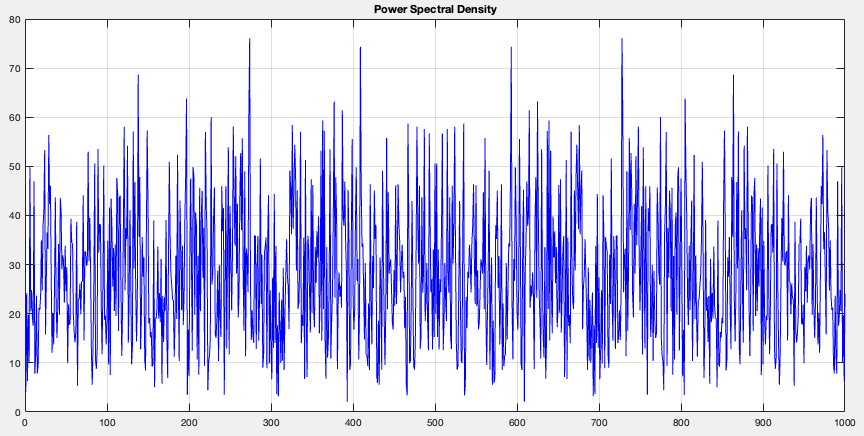
\includegraphics[width=0.95\textwidth]{seq2_1000_psd.png}
        \captionof{figure}{Sequence 2 PSD.}
      \end{minipage}
    \end{figure}

    \begin{figure}[H]
      \centering
      \begin{minipage}{0.5\textwidth}
        \centering
        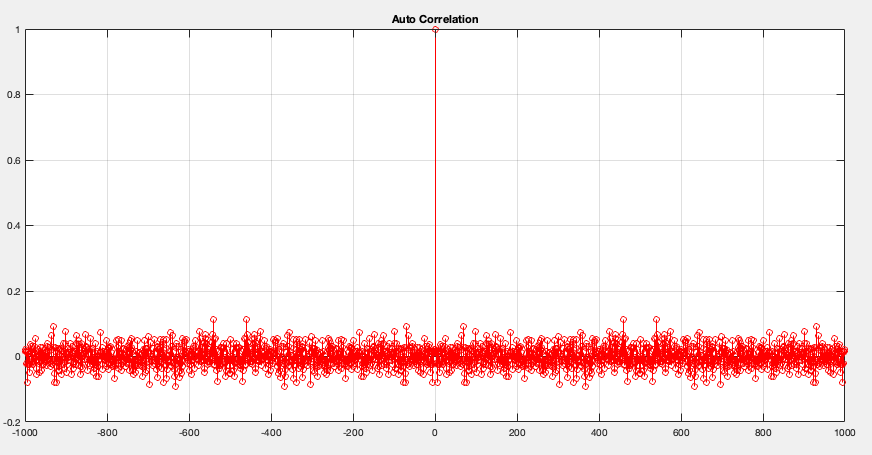
\includegraphics[width=0.95\textwidth]{seq1_1000_xcorr.png}
        \captionof{figure}{Sequence 1 Autocorrelation.}
      \end{minipage}%
      \begin{minipage}{0.5\textwidth}
        \centering
        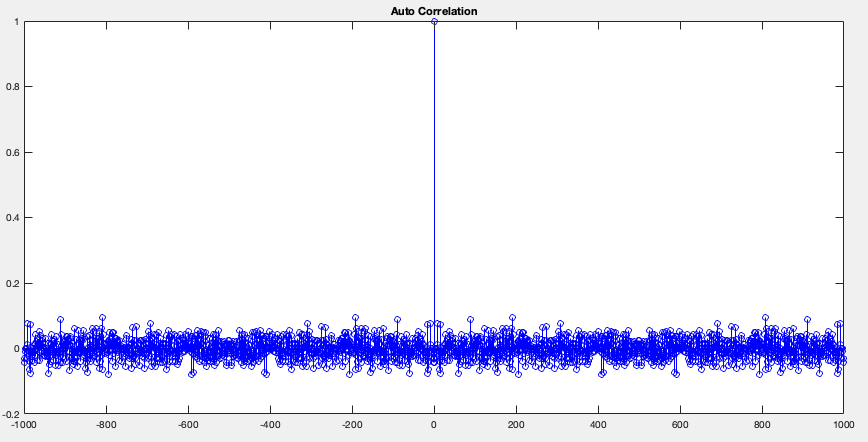
\includegraphics[width=0.95\textwidth]{seq2_1000_xcorr.png}
        \captionof{figure}{Sequence 2 Autocorrelation.}
      \end{minipage}
    \end{figure}

    \begin{figure}[H]
      \centering
      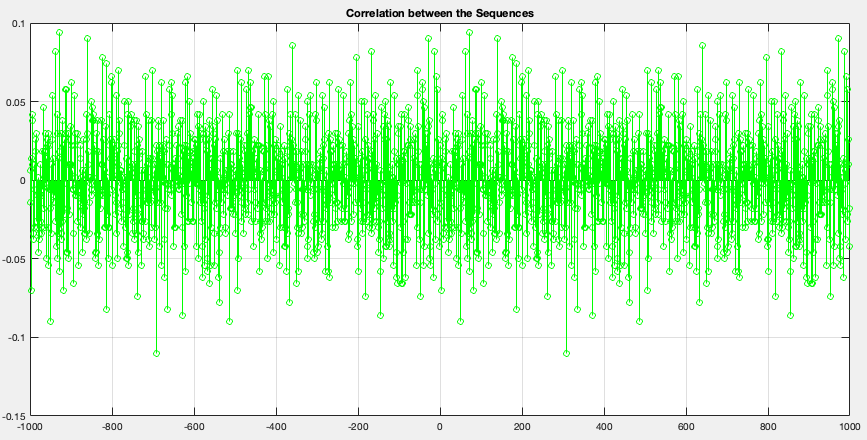
\includegraphics[width=0.5\textwidth]{xcorr_1000.png}
      \caption{Crosscorrelation of the Sequences.}
    \end{figure}

  %%
  % \vspace{16pt}
  \clearpage
  \section{Part 3}
    \subsection*
    {
      Generate 3 sequences 1000 long:
      \begin{enumerate}[-]
        \itemsep -6pt
        \item A = 3 + 3*randn(1000,1)
        \item B = 5 + 5*randn(1000,1)
        \item C = A + B
        \item DATA = [A B C]
      \end{enumerate}
      \begin{enumerate}[(a)]
        \itemsep -6pt
        \item Find the mean and variance for A, B, and C.
        \item Find the mean of DATA.
        \item Find the covariance of DATA.
      \end{enumerate}
    }

    \solution
    The mean, variance, and covariance can be easily calculated in MATLAB using 
    the $mean$, $var$, and $cov$ functions.
    \vspace{16pt}
    \begin{equation*}
      \begin{split}
        mean(A) &= 2.995996 \\
        mean(B) &= 5.080351 \\
        mean(C) &= 8.076347 \\
        mean(DATA) &= 5.384231 \\
        \\
        var(A) &= 8.941887 \\
        var(B) &= 26.113027 \\
        var(C) &= 33.745355 \\
        cov(DATA) &= \begin{bmatrix}
          8.941887 & -0.654780 & 8.287107 \\
          -0.654780 & 26.113027 & 25.458247 \\
          8.287107 & 25.458247 & 33.745355
        \end{bmatrix}
      \end{split}
    \end{equation*}

  %%
  % \vspace{16pt}
  \clearpage
  \section{Part 4}
    \subsection*
    {
      Develop the taylor series linearized approximation for the following 
      equation:
    }
    \begin{equation*}
        r(x,y) = \sqrt{(x-a)^2 + (y-b)^2}
    \end{equation*}
    
    \solution
    \vspace{12pt}
    Taking the partial derivatives with respect to x and y:
    \vspace{10pt}

    \begin{equation}
      \begin{split}
        \dfrac{\partial r}{\partial x} &= \dfrac{x - a}{\sqrt{(x-a)^2 + (y-b)^2}} \\[12pt]
        \dfrac{\partial r}{\partial y} &= \dfrac{y - b}{\sqrt{(x-a)^2 + (y-b)^2}}
      \end{split}
    \end{equation}

    \vspace{10pt}
    The first order approximation for a function of x and y takes the form:
    \vspace{-6pt}

    \begin{equation}
      r(x,y) = r(x_0,y_0) + \dfrac{\partial r}{\partial x}\Delta x + 
                            \dfrac{\partial r}{\partial y}\Delta y
    \end{equation}

    \begin{equation}  
      r(x,y) = \sqrt{(x_0-a)^2 + (y_0-b)^2} + 
                \dfrac{(x_0 - a)(x-x_0)}{\sqrt{(x_0-a)^2 + (y_0-b)^2}} + 
                \dfrac{(y_0 - b)(y-y_0)}{\sqrt{(x_0-a)^2 + (y_0-b)^2}}
    \end{equation}

\end{document}